\documentclass[10pt,a4paper]{article}

\usepackage[margin=18mm,top=16mm,bottom=18mm]{geometry}
\usepackage{graphicx}
\usepackage{booktabs}
\usepackage{tabularx}
\usepackage[dvipsnames]{xcolor}
\usepackage[colorlinks=true,linkcolor=NavyBlue,urlcolor=NavyBlue]{hyperref}
\usepackage{titlesec}
\usepackage{enumitem}
\usepackage{caption}
\usepackage{microtype}
\usepackage{parskip}

\titleformat{\section}{\large\bfseries}{\thesection.}{0.5em}{}
\titleformat{\subsection}{\normalsize\bfseries}{}{0em}{}
\titlespacing*{\section}{0pt}{12pt}{4pt}
\titlespacing*{\subsection}{0pt}{8pt}{2pt}

\setlist[itemize]{leftmargin=12pt,itemsep=2pt,topsep=3pt}
\captionsetup{font=small,labelfont=bf}
\newcolumntype{Y}{>{\raggedright\arraybackslash}X}

\title{\vspace{-12mm}\textbf{Multimodal Fashion \& Context Retrieval}}
\author{}
\date{}

\begin{document}
\maketitle
\vspace{-16mm}
{\small\itshape Compositional text-to-image retrieval over a fashion corpus.}
\vspace{2mm}

%======================================================================
\section{The problem}

CLIP is a strong zero-shot retrieval baseline and a weak compositional one. A dual
encoder pools an image into a single vector, so \textbf{red shirt + blue pants} and
\textbf{blue shirt + red pants} land in nearly the same place: the model registers
that \{red, blue, shirt, pants\} are present but loses \textbf{which colour attaches
to which garment}. This bag-of-words behaviour is well documented in contrastive
vision-language models, and it is the failure the brief's hint points at.

Every design decision below exists to fix attribute binding.

%======================================================================
\section{Approaches considered}

\begin{tabularx}{\textwidth}{@{}p{22mm}YY@{}}
\toprule
\textbf{Approach} & \textbf{Good when} & \textbf{Weakness} \\
\midrule
\textbf{A.} Vanilla CLIP, global vector
& Fast to build, genuinely zero-shot, scales trivially. The right default for coarse semantic search.
& No attribute binding. Fine-grained fashion vocabulary is weak (trained on web alt-text, not garments). \\
\addlinespace
\textbf{B.} Domain-tuned backbone
& One-line change; large gain on garment vocabulary and texture/fabric terms. Always worth doing.
& Still a dual encoder --- still pools the frame, so binding is unfixed. Domain shift if the corpus is not catalogue-like. \\
\addlinespace
\textbf{C.} Region multi-vector \emph{(chosen)}
& Directly attacks binding: a shirt crop contains only the shirt, so ``red'' cannot bind elsewhere. Still zero-shot.
& Index grows ${\sim}3\text{--}4\times$. Needs boxes --- annotations here, a detector at scale. Crops lose global context. \\
\addlinespace
\textbf{D.} Cross-encoder rerank
& Cross-attention resolves binding properly. Cheap if confined to a top-$k$ shortlist ($k{\approx}50$).
& Orders of magnitude slower per pair --- cannot touch the full corpus. Latency scales with $k$. \\
\addlinespace
\textbf{E.} Fine-tune with hard negatives
& Best ceiling; pushes binding into the vector so retrieval stays a single ANN lookup.
& Needs labelled attribute data (absent here), GPU budget, and sacrifices some zero-shot generality. \\
\bottomrule
\end{tabularx}

\vspace{3mm}
\textbf{Chosen: B + C}, with D scoped as the next increment. B is free. C is where the
brief's stated failure mode actually lives. D is deliberately deferred rather than
dropped --- it is the strongest precision lever left, and the shortlist architecture
already accepts it. E is out of reach: the dataset ships no attribute labels to train on.

%======================================================================
\section{Chosen architecture}

Modelled on \textbf{LookSync}, Glance's production visual product search system
(\href{https://arxiv.org/abs/2511.00072}{arXiv:2511.00072}): decompose the look into
layer-wise garment descriptions $\rightarrow$ vectorise $\rightarrow$ vector-DB
retrieval $\rightarrow$ rerank. The same four stages, adapted from \emph{product
retrieval given an AI-generated look} to \emph{scene retrieval given natural language}.

{\small\itshape LookSync's own bake-off put vanilla CLIP ViT-H/14 above FashionCLIP and
Fashion-SigLIP by 3--7\% MOS --- on catalogue product retrieval. That result did not
transfer here, which is why the backbone was chosen by measurement rather than
assumption (\S5).}

\subsection{Part A --- Indexer}

Two vector kinds per image:

\begin{center}\small
\begin{tabular}{@{}lll@{}}
\toprule
\textbf{Vector} & \textbf{Source} & \textbf{Answers} \\
\midrule
\texttt{global} & whole frame & scene (``inside a modern office''), vibe (``casual weekend'') \\
\texttt{region} & one per garment box & which colour belongs to which garment \\
\bottomrule
\end{tabular}
\end{center}

Region boxes are filtered to the 27 real garment/accessory categories. \textbf{46\% of
Fashionpedia's boxes are parts} --- sleeve, neckline, zipper, rivet --- and a crop of a
zipper is index noise. There is deliberately no third ``scene vector'': with a single
backbone that is just the global vector under another name. Storage is \textbf{ChromaDB},
per the brief's instruction to pick a convenient store rather than build one; the ML
logic is in \emph{what} is embedded, not the store.

\subsection{Part B --- Retriever}

\textbf{Decomposition is zero-shot by construction.} The brief grades handling of
``descriptions it hasn't seen explicitly in a training label'', which rules out the
obvious implementation. A parser with a hardcoded colour list and garment taxonomy
passes all five graded queries and silently drops any term outside its vocabulary ---
closed-vocabulary retrieval wearing a zero-shot costume. So no colours or garments are
ever enumerated:

\begin{itemize}
  \item \textbf{Split} on conjunctions and commas --- purely syntactic, no word list.
  \item \textbf{Route} each clause by comparing it against \emph{anchor prompts}
        describing what a garment is versus what a place is, using the text encoder
        itself. The encoder knows ``windbreaker'' even though we never wrote it down.
        Unsure clauses fall back to the global vector, so the system degrades to CLIP
        rather than to nothing.
\end{itemize}

\textbf{Binding via one-to-one assignment.} Region scoring alone is \emph{not} enough,
and this is the subtle part. If each clause independently takes its best-matching
region, then for an image with a \textbf{red shirt} and a \textbf{white tie}, the clause
``a red tie'' happily matches the red \emph{shirt} crop --- colour similarity dominates
garment identity, the swapped image still scores well, and nothing has been fixed.

Instead garment clauses are assigned to regions \textbf{one-to-one}, greedily by
descending similarity. Clauses compete: once ``a red tie'' claims the red crop, ``a
white shirt'' cannot also have it. An image genuinely containing a red tie and a white
shirt satisfies both clauses with two different crops; the colour-swapped image
satisfies neither well. This needs no category lookup, so it remains open-vocabulary.

{\small Fusion z-normalises per clause. Raw scores are not comparable across clauses or
backbones --- SigLIP's pairwise sigmoid loss puts its cosines on a completely different
scale from CLIP's InfoNCE (a random image scores $+0.18$ under CLIP, $-0.05$ under
SigLIP) --- so absolute thresholds would be meaningless.}

%======================================================================
\section{Dataset: built, not sampled}

\textbf{1{,}788 images} = 1{,}200 Fashionpedia + 588 COCO. Two audits drove this, and
both changed the design.

\subsection{Audit 1 --- Fashionpedia's distribution starves the graded queries}

\textbf{\texttt{tie} appears in 3 of 1{,}158 val images.} The compositional query ---
the one the entire architecture exists to win --- would have had essentially no ground
truth. Train is $39\times$ larger and holds 1{,}455 tie images and 1{,}402 tie+shirt
images, so the corpus is \textbf{stratified from train with a quota per graded query}
(200 tie+shirt, 200 formal, 180 outerwear, 160 shirt, 200 casual, 260 random
distractors), filled rarest-first so a tie+shirt image is never consumed by the
distractor bucket.

\subsection{Audit 2 --- Fashionpedia cannot serve the environment axis}

Zero-shot scene tagging found it is \textbf{85\% red carpet, runway and studio}. The
four environments the brief requires total \textbf{14.2\%} --- 19 office images and 4
home images out of 1{,}200 --- while three of the five graded queries are
environment-driven.

\begin{center}\small
\begin{tabular}{@{}lr@{}}
\toprule
\textbf{Scene} & \textbf{Share} \\
\midrule
red carpet & 36.2\% \\
runway / catwalk & 29.8\% \\
studio backdrop & 19.1\% \\
urban street / park / office / home & \textbf{14.2\%} $\leftarrow$ the required axis \\
\bottomrule
\end{tabular}
\end{center}

COCO fixes that, and does one thing a generic scene dataset could not: \textbf{its object
labels give scene ground truth that is not derived from CLIP}. A \texttt{bench} box is a
human annotation, so grading a CLIP retriever against it is not circular --- which
CLIP-generated scene tags could never be. Scene is inferred from co-present objects with
\texttt{person} always required: office $\leftarrow$ laptop/keyboard/mouse (89), home
$\leftarrow$ couch/bed/tv (175), park $\leftarrow$ bench (149), street $\leftarrow$
car/traffic light/bus (175).

{\small\itshape Honest limit: COCO rows carry no garment annotations, so they contribute a
global vector only. They are scene evidence and distractors, not garment evidence.}

%======================================================================
\section{Results}

\subsection{The metric}

Fashionpedia's HF release ships \textbf{no colour or scene attributes}, so there are no
labels to compute Precision@5 against. LookSync hit the same wall and fell back to human
Mean Opinion Score. So the headline metric needs no labels:

\begin{quote}\small
Retrieve top-5 for \emph{``a red tie and a white shirt''}, then for \emph{``a white tie
and a red shirt''}. Both queries contain an \textbf{identical bag of words}. A system
that ignores binding returns nearly the same images for both (overlap $\rightarrow$ 1.0).
A system that binds returns different ones (overlap $\rightarrow$ 0).
\end{quote}

\textbf{Lower is better.} The metric is rank-based (no score comparability needed) and
self-supervised (no ground truth needed): it measures \emph{sensitivity to binding},
exactly the property the brief's hint calls out. Averaged over 4 swap pairs, $k=5$.

\begin{figure}[h]
\centering
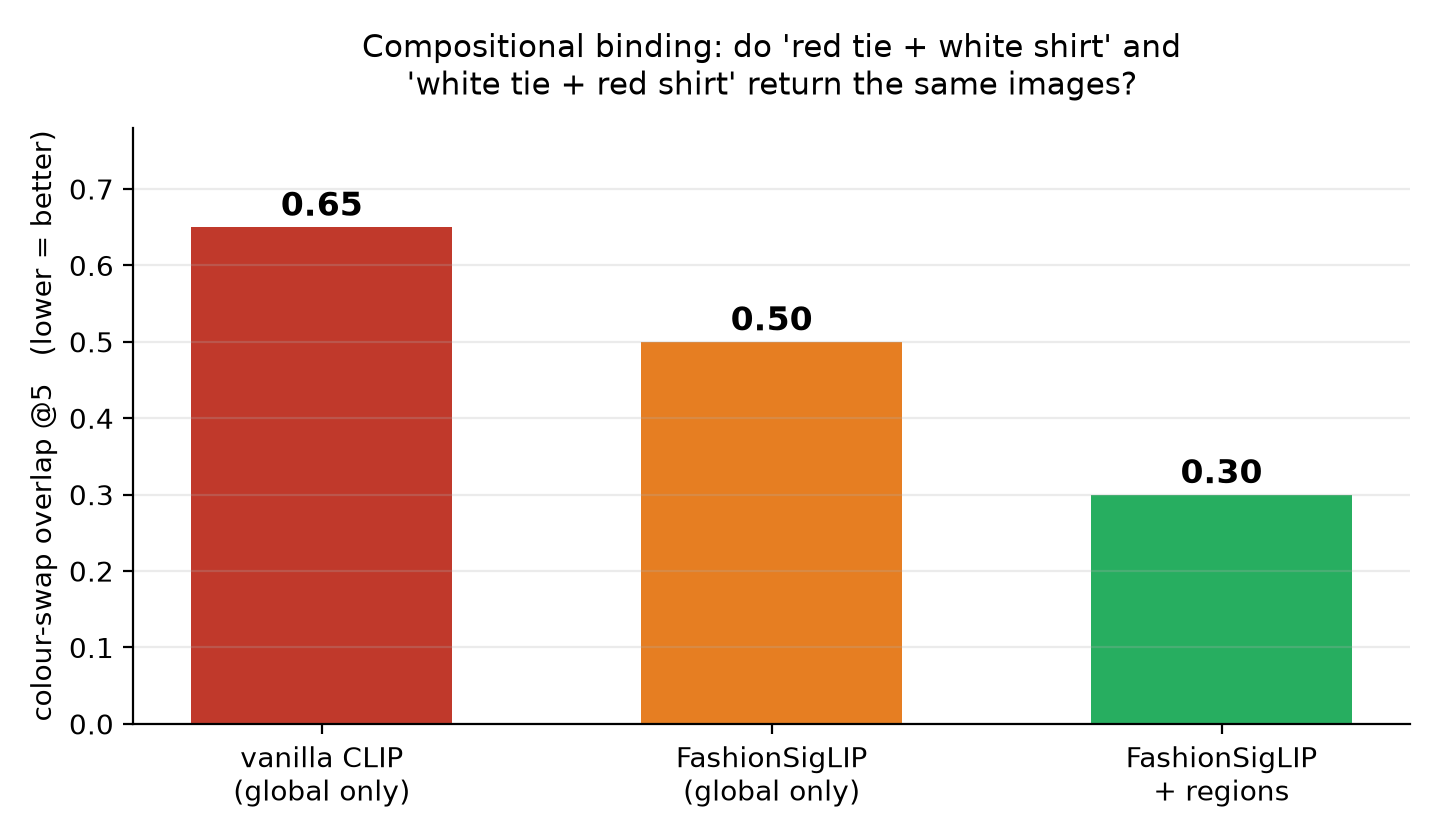
\includegraphics[width=0.72\textwidth]{eval/ablation.png}
\end{figure}

\vspace{-2mm}
\begin{center}\small
\begin{tabular}{@{}lcl@{}}
\toprule
\textbf{Configuration} & \textbf{Swap overlap} $\downarrow$ & \textbf{Reading} \\
\midrule
vanilla CLIP (global only) & 0.65 & Returns 65\% the same images either way. \\
FashionSigLIP (global only) & 0.50 & Domain vocabulary helps; pooling still destroys binding. \\
\textbf{FashionSigLIP + regions} & \textbf{0.30} & Region scoring + assignment does the work. \\
\bottomrule
\end{tabular}
\end{center}

The backbone swap buys $0.65 \rightarrow 0.50$; \textbf{the mechanism buys $0.50
\rightarrow 0.30$}. That split matters: the gain is attributable to the architecture,
not to having picked a fancier model.

\subsection{Zero-shot check}

The direct test is a query built from words that appear \emph{nowhere} in the codebase:

\begin{quote}
\texttt{python query.py "a burnt sienna windbreaker" -{}-k 3}
\end{quote}

The clause routes to \textsc{garment} (margin $+0.0375$) and the top-3 are all
burnt-orange outerwear: a rust quilted bomber, a rust jacket-and-trouser set, a
burnt-orange fur jacket. Routing is a similarity comparison against role anchors, so the
vocabulary is whatever the backbone knows. A hardcoded parser would have dropped both
terms and silently returned noise.

\subsection{Relevance: swap overlap alone is not sufficient}

Swap overlap measures whether a system is \emph{sensitive} to binding, not whether it is
\emph{right}. A retriever returning five random images would score a perfect 0.00.
Adding region vectors adds noise, and noise also lowers overlap --- so the result above
is consistent with better binding \emph{and} with simply being noisier. The two must be
disentangled, and the only way to do that here is to look at the output.

Precision@5, judged by inspection of the top-5 for each graded query. An image counts
only if it satisfies \emph{every} attribute the query names (contact sheets for both
systems are in the repo under \texttt{eval/}):

\begin{center}\small
\begin{tabular}{@{}lcc@{}}
\toprule
\textbf{Graded query} & \textbf{Ours} & \textbf{Vanilla CLIP} \\
\midrule
1. A person in a bright yellow raincoat & 2/5 & 1/5 \\
2. Professional business attire inside a modern office & 4/5 & 2/5 \\
3. Someone wearing a blue shirt sitting on a park bench & 3/5 & 1/5 \\
4. Casual weekend outfit for a city walk & 5/5 & 4/5 \\
5. A red tie and a white shirt in a formal setting & \textbf{4/5} & \textbf{0/5} \\
\midrule
\textbf{Precision@5} & \textbf{0.72} & \textbf{0.32} \\
\bottomrule
\end{tabular}
\end{center}

Relevance moves the same way as binding: the region system is not merely \emph{different}
from CLIP, it is better --- and by a wider margin on the compositional query than
anywhere else, which is exactly where the architecture was aimed. It is worth seeing
rather than reading:

\begin{figure}[h]
\centering
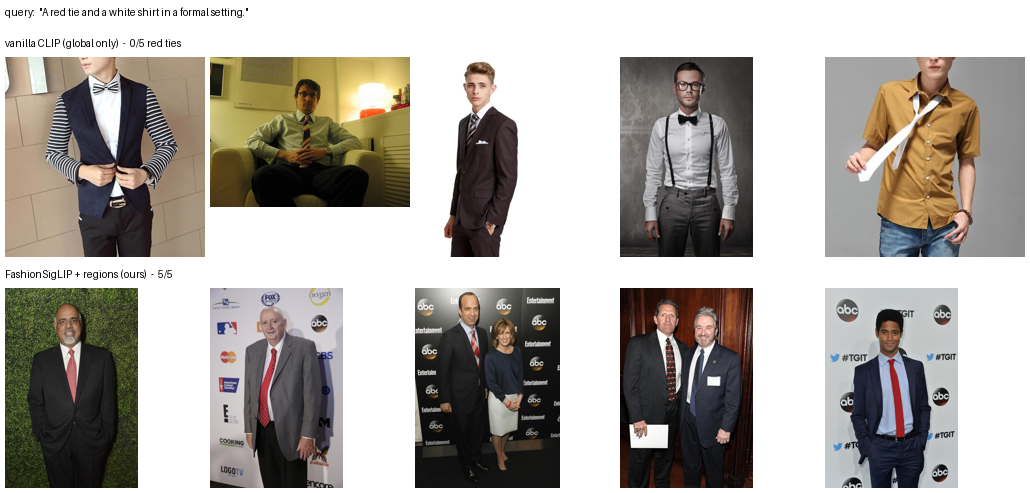
\includegraphics[width=\textwidth]{eval/comparison_compositional.png}
\end{figure}

\vspace{-3mm}
{\small Vanilla CLIP returns \textbf{zero red ties}: a white bow tie, an olive tie, a
striped tie, a black bow tie, and --- the diagnostic case --- \textbf{a white tie on a
gold shirt}. The colour-swapped image is retrieved as a top match, because a pooled
vector registers \{red, white, tie, shirt\} without binding. This is the brief's hint,
reproduced exactly.}

\subsection{Known limitations}

\begin{itemize}\small
  \item \textbf{Query 1 is the weakest (2/5).} Fashionpedia has no \texttt{raincoat}
        category --- only coat/jacket/cape --- so ``raincoat'' degrades to ``yellow
        garment'' and the tail drifts to yellow tops and an orange dress. A vocabulary
        gap in the corpus, not in the model.
  \item \textbf{Precision@5 was judged by the author on 25 image-query pairs.} Small and
        non-blind. Scores move with rubric strictness, and honestly so: query 5 is scored
        4/5, with one clear miss (a red-and-white \emph{striped} tie over a light blue
        shirt) and two borderline results (a navy tie with red motifs; a red tie over a
        pale blue shirt). Read strictly it is 2/5; read generously, 5/5. Query 2 is 4/5
        generously and 2/5 if both business attire \emph{and} an office are required. The
        gap survives every rubric, because vanilla CLIP returns \textbf{zero} red ties
        under any reading.
  \item \textbf{4 swap pairs is a small sample.} The ordering is consistent and the gap
        wide, but absolute values carry meaningful variance.
  \item \textbf{Greedy assignment, not Hungarian.} Optimal for ${\le}5$ clauses in
        practice, but not guaranteed.
  \item \textbf{Region boxes come from annotations.} At 1M images this needs a detector
        (LookSync uses SAM v2 + Florence as its fallback path), introducing detector
        error the current numbers exclude.
  \item \textbf{Query 4 does not decompose} --- ``Casual weekend outfit for a city walk''
        routes as a single garment clause, since the splitter has no rule for
        ``for a\ldots''. It scores 5/5 anyway because the whole-query prior still
        carries the city context: the fallback path saved it, which is luck, not design.
\end{itemize}

%======================================================================
\section{Scalability to 1M images}

Candidate generation is an ANN lookup in ChromaDB over the whole corpus; only the
shortlist is scored densely. Cost is $O(\log N)$ in corpus size, so the retrieval logic
is unchanged at 1M images. Three real costs:

\begin{itemize}
  \item \textbf{Index size grows ${\sim}3.4\times$} (6{,}036 vectors for 1{,}788 images).
        At 1M images that is ${\sim}3.4$M vectors $\times$ 768 dims $\times$ 4 bytes
        $\approx$ 10\,GB --- past comfortable RAM. Fix: product quantisation, or index
        regions only for garment-bearing images.
  \item \textbf{Dense scoring is $O(\text{candidates} \times \text{clauses} \times
        \text{regions})$}, but candidates are capped at ${\sim}150$/clause, so this is
        constant in $N$.
  \item \textbf{Chroma is the right call at this scale and the wrong one at 1M.} The
        brief says to pick the convenient store; the migration path is Qdrant or Vertex
        AI Vector Search (LookSync serves 18M+ products at P90 $<$ 1\,s with an
        offline-index / online-serve split plus aggressive caching).
\end{itemize}

%======================================================================
\section{Future work}

\subsection{(a) Adding locations (cities, places) and weather}

The architecture already has the right seam: \textbf{scene clauses route to the global
vector}, so location and weather are a third clause role rather than a redesign.

\begin{itemize}
  \item \textbf{Add a role, not a model.} Extend the anchor set with ``a city or
        geographic location'' and ``the weather or time of day''. Routing is
        similarity-based, so this is additive --- no retraining, no vocabulary.
  \item \textbf{Cheap metadata first.} EXIF GPS and capture time give city and season for
        free where present; both become Chroma metadata filters, which cut the candidate
        set \emph{before} any vector work and so cost nothing at query time.
  \item \textbf{Where labels are absent, use a dedicated encoder.} A geo-aware model
        (StreetCLIP was trained for exactly this) tags city/region; weather is well
        within zero-shot CLIP (``an overcast day'', ``a rain-soaked street''). Store as a
        fourth vector kind plus metadata.
  \item \textbf{Weather is a garment prior, not just a filter} --- the commercially
        interesting part. ``What to wear in Bangalore in July'' is a monsoon query: it
        should surface raincoats and closed shoes. That is a learned correlation between
        weather and garment category, not a retrieval constraint, and it is where a
        recommendation layer would sit on top of this retriever.
\end{itemize}

\subsection{(b) Improving precision}

\begin{itemize}
  \item \textbf{Cross-encoder rerank (approach D) is the biggest lever left.} BLIP-ITM
        over the top-50: cross-attention resolves binding properly rather than
        approximating it with assignment. Confined to a shortlist it is affordable, and
        the architecture already produces that shortlist. This is the first thing I would
        build next.
  \item \textbf{Hard-negative mining.} Colour-swapped and garment-swapped negatives are
        exactly what the swap metric measures --- mine them automatically from the corpus
        and fine-tune (approach E). This pushes binding into the embedding so it survives
        at ANN time instead of being reconstructed at scoring time.
  \item \textbf{Replace the syntactic splitter with an LLM decomposer}, as LookSync does.
        It fixes the query-4 failure directly and handles possessives, negation (``not
        black'') and implicit garments (``business attire'' $\rightarrow$ blazer +
        button-down) that regex cannot.
  \item \textbf{Learn the fusion weights.} \texttt{W\_PRIOR} and the clause weights are
        hand-set. With even a few hundred judged pairs they should be fit, not guessed.
  \item \textbf{Detector-based regions.} Removes the annotation dependency and lets region
        scoring work on arbitrary images --- required to run on real traffic.
\end{itemize}

%======================================================================
\section{Codebase}

\begin{center}
\href{https://github.com/Avishi03/glance-fashion-retrieval}{\texttt{github.com/Avishi03/glance-fashion-retrieval}}
\end{center}

Part B entrypoint --- accepts a natural-language string, returns the top-$k$ images:

\begin{quote}\small
\texttt{python query.py "A red tie and a white shirt in a formal setting." -{}-k 5}\\
\texttt{python query.py "a burnt sienna windbreaker" -{}-show}\\
\texttt{python query.py "a blue shirt in a park" -{}-backbone vanilla-clip -{}-no-regions}
\end{quote}

It prints the clause decomposition alongside the ranked results, so routing decisions are
inspectable. The \texttt{-{}-backbone} / \texttt{-{}-no-regions} flags make the ablation
in \S5 reproducible from the command line.

{\small \texttt{data/} corpus construction + audits \quad$\cdot$\quad \texttt{indexer/}
Part A: encoders, crops, vector storage \quad$\cdot$\quad \texttt{retriever/} Part B:
decomposition, routing, assignment, fusion \quad$\cdot$\quad \texttt{eval/} graded
queries + stress test. Logic is separated from data throughout: the corpus is JSON +
images, every model is swappable by a flag, and the eval harness runs any
backbone/config combination without touching retrieval code.}

\end{document}
